\section{Vertiefung: Prolog ausprobieren}

Mit Hilfe der Online-Prolog-Umgebung\cite{prolog-online} wurde folgendes ausprobiert, um ein Gef�hl f�r die Programmierung in Prolog zu bekommen:

\paragraph{Einfaches Beispiel f�r Beziehungen mit Prolog}

\begin{lstlisting}
%facts
likes(dan,sally).
likes(sally,dan).
likes(josh, brittney).
likes(sally, brittney).

hates(josh, dan).
hates(dan, josh).
hates(brittney, sally).

friendship(X,Y):-
    likes(X,Y),
    likes(Y,X).

enemies(X,Y):-
    hates(X,Y),
    hates(Y,X).

misunderstanding(X,Y):-
    hates(X,Y),likes(Y,X);
    hates(Y,X),likes(X,Y);
\end{lstlisting}

\begin{figure}[H]
    \centering
    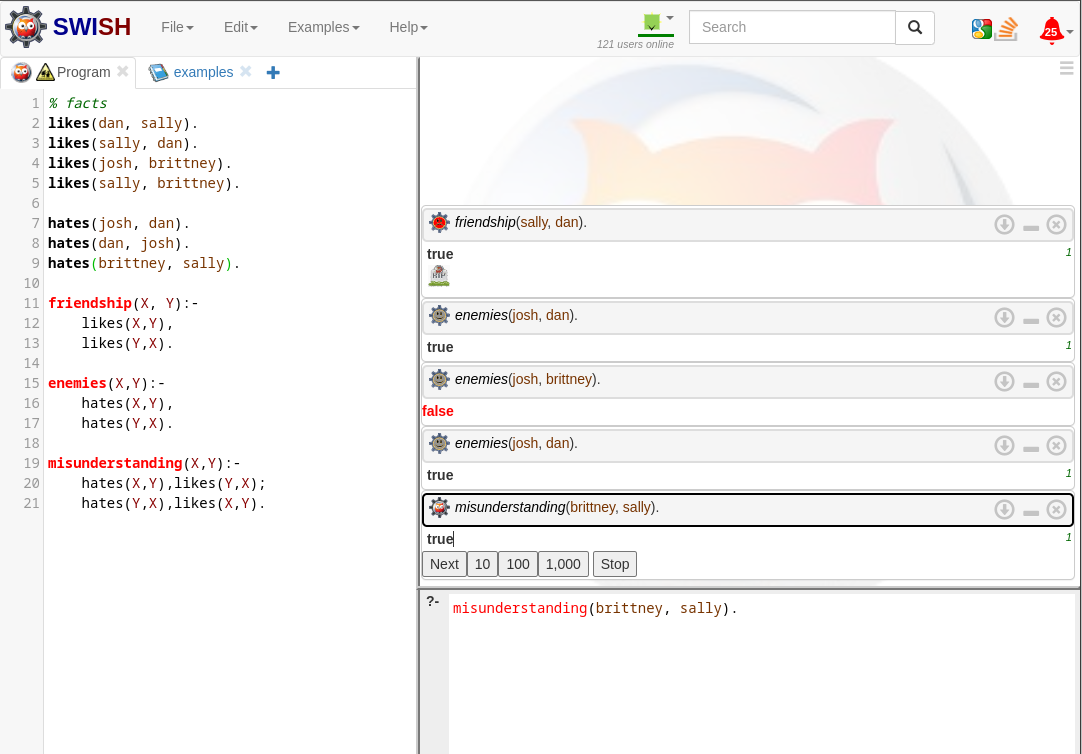
\includegraphics[width=\textwidth]{figures/kap8/prolog-relationships.png}
    \caption{Einfaches Modell von Beziehungen mit Prolog}
    \label{fig:prolog-relationships}
\end{figure}

\paragraph{Ein eher faktenbasiertes Beispiel}

\begin{lstlisting}
fond_of_humans(cat).
fond_of_humans(dog).

comfortable_in_houses(cat).
comfortable_in_houses(dog).

breeds_easily_in_captivity(cat).
breeds_easily_in_captivity(dog).
breeds_easily_in_captivity(chicken).
breeds_easily_in_captivity(cow).
breeds_easily_in_captivity(horse).
breeds_easily_in_captivity(ox).

grows_quickly(chicken).
grows_quickly(cow).

useful_animal(horse).
useful_animal(ox).
useful_animal(dog).

is_pet(X):-
    fond_of_humans(X),
    comfortable_in_houses(Y).

is_farmed(X):-
    breeds_easily_in_captivity(X),
    grows_quickly(X).

is_work_animal(X):-
    breeds_easily_in_captivity(X),
    useful_animal(X).
\end{lstlisting}

\begin{figure}[H]
    \centering
    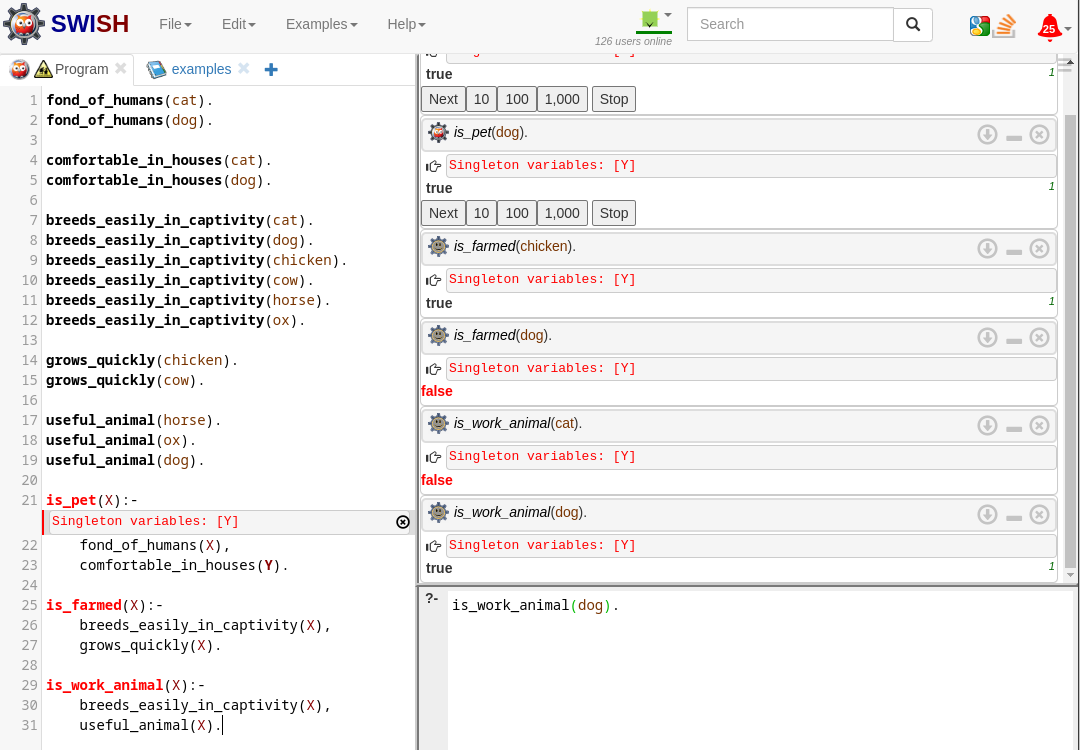
\includegraphics[width=\textwidth]{figures/kap8/prolog-animals.png}
    \caption{Einfaches Modell von Tieren mit Prolog}
    \label{fig:prolog-animals}
\end{figure}